\documentclass{article}
\usepackage[UTF8]{ctex}
\usepackage[T1]{fontenc}
\usepackage[utf8]{inputenc}
\usepackage{titlesec}
\usepackage{xcolor}
\usepackage[colorlinks, linkcolor = black]{hyperref}
\usepackage{tikz}
\usepackage{mathpazo}
\usepackage{subfigure}
\usepackage{amsmath}
\usepackage{amsthm}
\usepackage{amssymb}
\usepackage{enumerate}
\usepackage{geometry}
\usetikzlibrary{positioning}
\usetikzlibrary[arrows, shapes, chains]
\newcounter{row}
\newcounter{col}

\newcommand\setrow[3]{
  \setcounter{col}{1}
  \foreach \n in {#1, #2, #3} {
    \edef\x{\value{col} - 0.5}
    \edef\y{3.5 - \value{row}}
    \node[anchor = center] at (\x, \y) {\n};
    \stepcounter{col}
  }
  \stepcounter{row}
}

\titleformat{\section}[block]{\LARGE\scshape}{\arabic{section}}{1em}{}[]

\tikzset{
    normal/.style = {ellipse, draw = black, text ragged, minimum width = 6em, scale = 0.5},
    expand/.style = {ellipse, draw = red!70!black, text ragged, minimum width = 6em, black, fill = red!30!white, scale = 0.5},
    length/.style = {text ragged, scale = 0.4},
    level distance = 5em,
    level 1/.style = {sibling distance = 60em},
    level 2/.style = {sibling distance = 30em},
    level 3/.style = {sibling distance = 20em},
    level 4/.style = {sibling distance = 8em},
    level 5/.style = {sibling distance = 10em}
}

\title{Homework 2}
\author{PB17000297 罗晏宸}
\date{March 8 2020}

\begin{document}
\maketitle

\section{Exercise 3.6}
跟踪A$^*$算法应用直线距离启发式求解从 Lugoj 到 Bucharest 问题的过程。给出结点扩展的顺序和每个结点的$f$、$g$ 和 $h$ 值。

\paragraph{解}
Romania 问题中到 Bucharest 的直线距离如表所示:
\begin{table}[h]
    \centering
    \begin{tabular}{lrlr}
    \textbf{Arad}      & 366 & \textbf{Mehadia}        & 241 \\
    \textbf{Bucharest} & 0   & \textbf{Neamt}          & 234 \\
    \textbf{Craiova}   & 160 & \textbf{Oradea}         & 380 \\
    \textbf{Drobeta}   & 242 & \textbf{Pitesti}        & 100 \\
    \textbf{Eforie}    & 161 & \textbf{Rimnicu Vilcea} & 193 \\
    \textbf{Fagaras}   & 176 & \textbf{Sibiu}          & 253 \\
    \textbf{Giurgiu}   & 77  & \textbf{Timisoara}      & 329 \\
    \textbf{Hirsova}   & 151 & \textbf{Urziceni}       & 80  \\
    \textbf{Iasi}      & 226 & \textbf{Vaslui}         & 199 \\
    \textbf{Lugoj}     & 244 & \textbf{Zerind}         & 374
    \end{tabular}
    \caption{$h_{SLD}$的值——到 Bucharest 的直线距离}
\end{table}

使用直线距离启发式,应用A$^*$算法,过程如下:
\newgeometry{left = 1cm, right = 1cm, top = 0cm, bottom = 0.5cm}
\begin{figure}
    \centering

    \subfigure
    {
        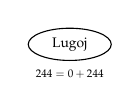
\begin{tikzpicture}[scale = 0.45]
            \node [normal] (L) {Lugoj};

            \node [length, below = 0.2em of L] (dL) {$244 = 0 + 244$};
        \end{tikzpicture}
    }

    \subfigure
    {
        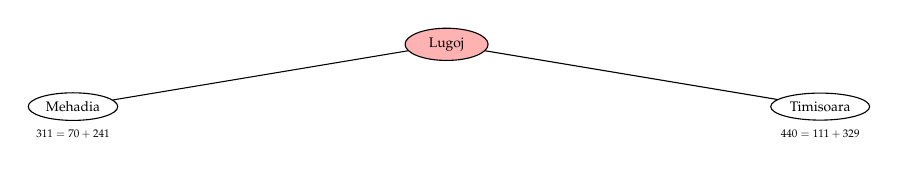
\begin{tikzpicture}[scale = 0.45]
            \node [expand] (L) {Lugoj}
                child {node [normal] (M) {Mehadia}}
                child {node [normal] (T) {Timisoara}};

            \node [length, below = 0.2em of M] (dM) {$311 = 70 + 241$};
            \node [length, below = 0.2em of T] (dT) {$440 = 111 + 329$};
        \end{tikzpicture}
    }

    \subfigure
    {
        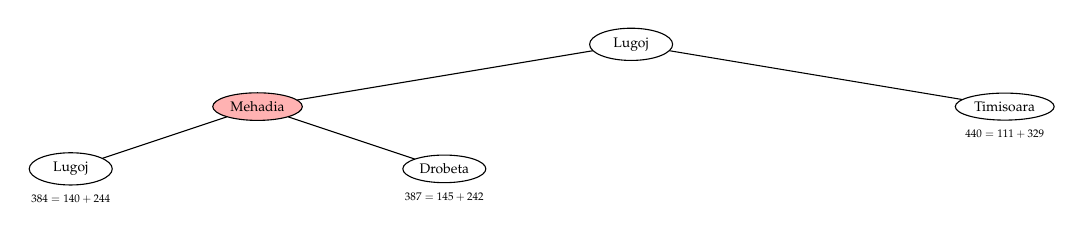
\begin{tikzpicture}[scale = 0.45]
            \node [normal] (L) {Lugoj}
                child {node [expand] (M) {Mehadia}
                    child {node [normal] (L2) {Lugoj}}
                    child {node [normal] (D) {Drobeta}}
                }
                child {node [normal] (T) {Timisoara}};

            \node [length, below = 0.2em of L2] (dL) {$384 = 140 + 244$};
            \node [length, below = 0.2em of D] (dD) {$387 = 145 + 242$};
            \node [length, below = 0.2em of T] (dT) {$440 = 111 + 329$};
        \end{tikzpicture}
    }

    \subfigure
    {
        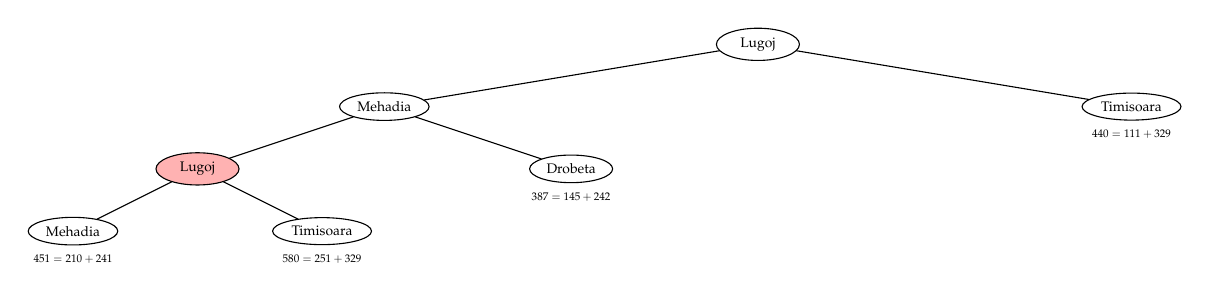
\begin{tikzpicture}[scale = 0.45]
            \node [normal] (L) {Lugoj}
                child {node [normal] (M) {Mehadia}
                    child {node [expand] (L2) {Lugoj}
                        child {node [normal] (M2) {Mehadia}}
                        child {node [normal] (T2) {Timisoara}}
                    }
                    child {node [normal] (D) {Drobeta}}
                }
                child {node [normal] (T) {Timisoara}};

            \node [length, below = 0.2em of M2] (dM2) {$451 = 210 + 241$};
            \node [length, below = 0.2em of T2] (dT2) {$580 = 251 + 329$};
            \node [length, below = 0.2em of D] (dD) {$387 = 145 + 242$};
            \node [length, below = 0.2em of T] (dT) {$440 = 111 + 329$};
        \end{tikzpicture}
    }

    \subfigure
    {
        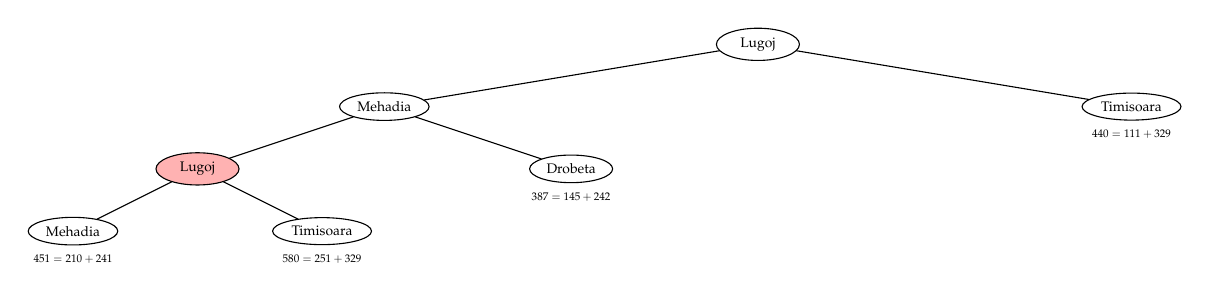
\begin{tikzpicture}[scale = 0.45]
            \node [normal] (L) {Lugoj}
                child {node [normal] (M) {Mehadia}
                    child {node [expand] (L2) {Lugoj}
                        child {node [normal] (M2) {Mehadia}}
                        child {node [normal] (T2) {Timisoara}}
                    }
                    child {node [normal] (D) {Drobeta}}
                }
                child {node [normal] (T) {Timisoara}};

            \node [length, below = 0.2em of M2] (dM2) {$451 = 210 + 241$};
            \node [length, below = 0.2em of T2] (dT2) {$580 = 251 + 329$};
            \node [length, below = 0.2em of D] (dD) {$387 = 145 + 242$};
            \node [length, below = 0.2em of T] (dT) {$440 = 111 + 329$};
        \end{tikzpicture}
    }

    \subfigure
    {
        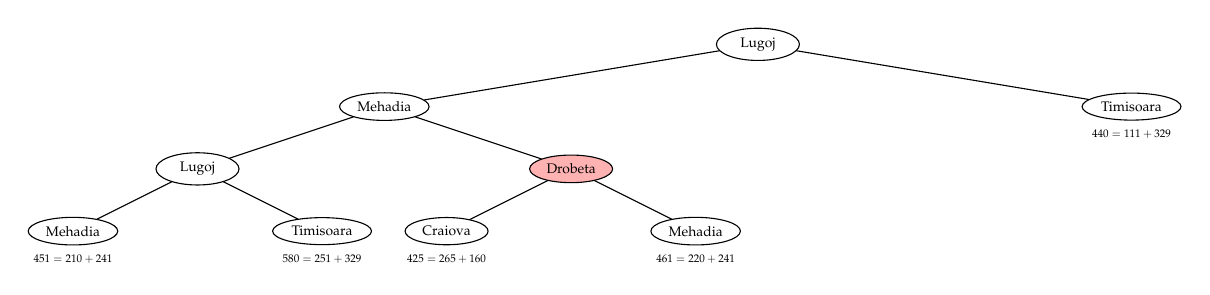
\begin{tikzpicture}[scale = 0.45]
            \node [normal] (L) {Lugoj}
                child {node [normal] (M) {Mehadia}
                    child {node [normal] (L2) {Lugoj}
                        child {node [normal] (M2) {Mehadia}}
                        child {node [normal] (T2) {Timisoara}}
                    }
                    child {node [expand] (D) {Drobeta}
                        child {node [normal] (C) {Craiova}}
                        child {node [normal] (M3) {Mehadia}}
                    }
                }
                child {node [normal] (T) {Timisoara}};

            \node [length, below = 0.2em of M2] (dM2) {$451 = 210 + 241$};
            \node [length, below = 0.2em of T2] (dT2) {$580 = 251 + 329$};
            \node [length, below = 0.2em of M3] (dM3) {$461 = 220 + 241$};
            \node [length, below = 0.2em of C] (dC) {$425 = 265 + 160$};
            \node [length, below = 0.2em of T] (dT) {$440 = 111 + 329$};
        \end{tikzpicture}
    }

    \subfigure
    {
        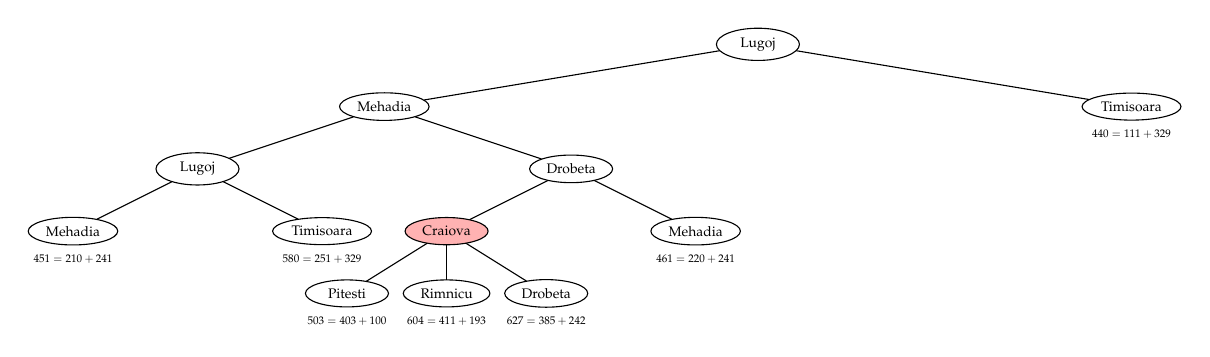
\begin{tikzpicture}[scale = 0.45]
            \node [normal] (L) {Lugoj}
                child {node [normal] (M) {Mehadia}
                    child {node [normal] (L2) {Lugoj}
                        child {node [normal] (M2) {Mehadia}}
                        child {node [normal] (T2) {Timisoara}}
                    }
                    child {node [normal] (D) {Drobeta}
                        child {node [expand] (C) {Craiova}
                            child {node [normal] (P) {Pitesti}}
                            child {node [normal] (R) {Rimnicu}}
                            child {node [normal] (D2) {Drobeta}}
                        }
                        child {node [normal] (M3) {Mehadia}}
                    }
                }
                child {node [normal] (T) {Timisoara}};

            \node [length, below = 0.2em of M2] (dM2) {$451 = 210 + 241$};
            \node [length, below = 0.2em of T2] (dT2) {$580 = 251 + 329$};
            \node [length, below = 0.2em of M3] (dM3) {$461 = 220 + 241$};
            \node [length, below = 0.2em of P] (dP) {$503 = 403 + 100$};
            \node [length, below = 0.2em of R] (dR) {$604 = 411 + 193$};
            \node [length, below = 0.2em of D2] (dD2) {$627 = 385 + 242$};
            \node [length, below = 0.2em of T] (dT) {$440 = 111 + 329$};
        \end{tikzpicture}
    }
    \caption{使用A$^*$搜索应用直线距离启发式求解从 Lugoj 到 Bucharest 问题}
    \label{figure:1}
\end{figure}

\begin{figure}[h]
    \centering
    \subfigure
    {
        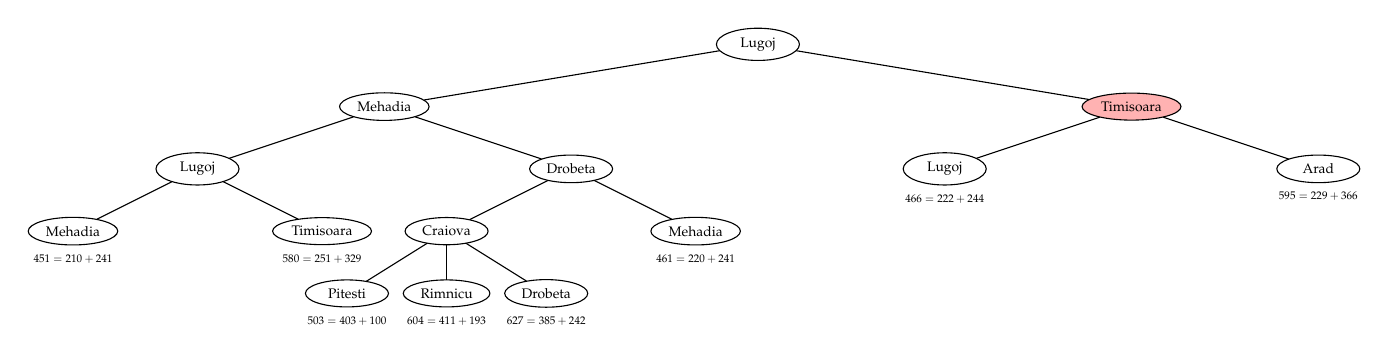
\begin{tikzpicture}[scale = 0.45]
            \node [normal] (L) {Lugoj}
                child {node [normal] (M) {Mehadia}
                    child {node [normal] (L2) {Lugoj}
                        child {node [normal] (M2) {Mehadia}}
                        child {node [normal] (T2) {Timisoara}}
                    }
                    child {node [normal] (D) {Drobeta}
                        child {node [normal] (C) {Craiova}
                            child {node [normal] (P) {Pitesti}}
                            child {node [normal] (R) {Rimnicu}}
                            child {node [normal] (D2) {Drobeta}}
                        }
                        child {node [normal] (M3) {Mehadia}}
                    }
                }
                child {node [expand] (T) {Timisoara}
                    child {node [normal] (L3) {Lugoj}}
                    child {node [normal] (A) {Arad}}
                };

            \node [length, below = 0.2em of M2] (dM2) {$451 = 210 + 241$};
            \node [length, below = 0.2em of T2] (dT2) {$580 = 251 + 329$};
            \node [length, below = 0.2em of M3] (dM3) {$461 = 220 + 241$};
            \node [length, below = 0.2em of P] (dP) {$503 = 403 + 100$};
            \node [length, below = 0.2em of R] (dR) {$604 = 411 + 193$};
            \node [length, below = 0.2em of D2] (dD2) {$627 = 385 + 242$};
            \node [length, below = 0.2em of L3] (dL3) {$466 = 222 + 244$};
            \node [length, below = 0.2em of A] (dA) {$595 = 229 + 366$};
        \end{tikzpicture}
    }

    \subfigure
    {
        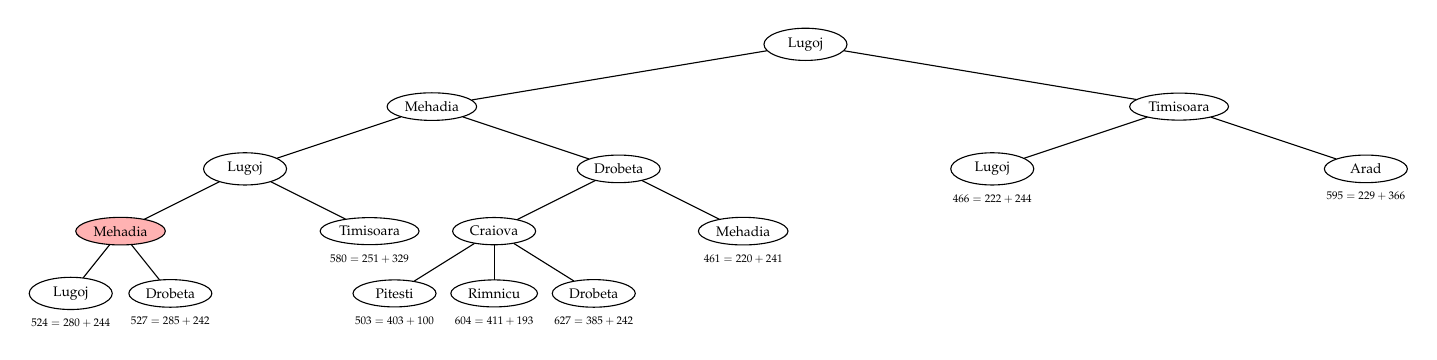
\begin{tikzpicture}[scale = 0.45]
            \node [normal] (L) {Lugoj}
                child {node [normal] (M) {Mehadia}
                    child {node [normal] (L2) {Lugoj}
                        child {node [expand] (M2) {Mehadia}
                            child {node [normal] (L4) {Lugoj}}
                            child {node [normal] (D3) {Drobeta}}
                        }
                        child {node [normal] (T2) {Timisoara}}
                    }
                    child {node [normal] (D) {Drobeta}
                        child {node [normal] (C) {Craiova}
                            child {node [normal] (P) {Pitesti}}
                            child {node [normal] (R) {Rimnicu}}
                            child {node [normal] (D2) {Drobeta}}
                        }
                        child {node [normal] (M3) {Mehadia}}
                    }
                }
                child {node [normal] (T) {Timisoara}
                    child {node [normal] (L3) {Lugoj}}
                    child {node [normal] (A) {Arad}}
                };

            \node [length, below = 0.2em of L4] (dL4) {$524 = 280 + 244$};
            \node [length, below = 0.2em of D3] (dD3) {$527 = 285 + 242$};
            \node [length, below = 0.2em of T2] (dT2) {$580 = 251 + 329$};
            \node [length, below = 0.2em of M3] (dM3) {$461 = 220 + 241$};
            \node [length, below = 0.2em of P] (dP) {$503 = 403 + 100$};
            \node [length, below = 0.2em of R] (dR) {$604 = 411 + 193$};
            \node [length, below = 0.2em of D2] (dD2) {$627 = 385 + 242$};
            \node [length, below = 0.2em of L3] (dL3) {$466 = 222 + 244$};
            \node [length, below = 0.2em of A] (dA) {$595 = 229 + 366$};
        \end{tikzpicture}
    }

    \subfigure
    {
        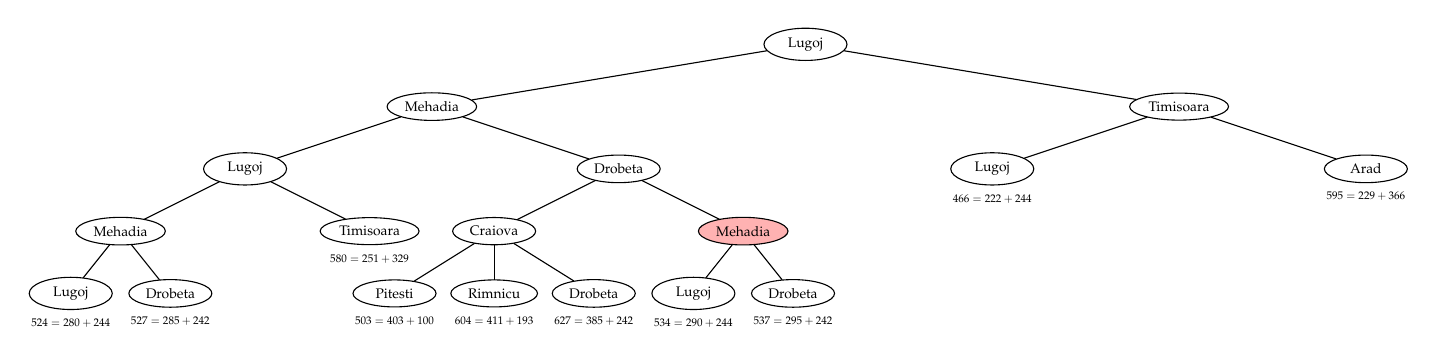
\begin{tikzpicture}[scale = 0.45]
            \node [normal] (L) {Lugoj}
                child {node [normal] (M) {Mehadia}
                    child {node [normal] (L2) {Lugoj}
                        child {node [normal] (M2) {Mehadia}
                            child {node [normal] (L4) {Lugoj}}
                            child {node [normal] (D3) {Drobeta}}
                        }
                        child {node [normal] (T2) {Timisoara}}
                    }
                    child {node [normal] (D) {Drobeta}
                        child {node [normal] (C) {Craiova}
                            child {node [normal] (P) {Pitesti}}
                            child {node [normal] (R) {Rimnicu}}
                            child {node [normal] (D2) {Drobeta}}
                        }
                        child {node [expand] (M3) {Mehadia}
                            child {node [normal] (L5) {Lugoj}}
                            child {node [normal] (D4) {Drobeta}}
                        }
                    }
                }
                child {node [normal] (T) {Timisoara}
                    child {node [normal] (L3) {Lugoj}}
                    child {node [normal] (A) {Arad}}
                };

            \node [length, below = 0.2em of L4] (dL4) {$524 = 280 + 244$};
            \node [length, below = 0.2em of D3] (dD3) {$527 = 285 + 242$};
            \node [length, below = 0.2em of T2] (dT2) {$580 = 251 + 329$};
            \node [length, below = 0.2em of L5] (dL5) {$534 = 290 + 244$};
            \node [length, below = 0.2em of D4] (dD4) {$537 = 295 + 242$};
            \node [length, below = 0.2em of P] (dP) {$503 = 403 + 100$};
            \node [length, below = 0.2em of R] (dR) {$604 = 411 + 193$};
            \node [length, below = 0.2em of D2] (dD2) {$627 = 385 + 242$};
            \node [length, below = 0.2em of L3] (dL3) {$466 = 222 + 244$};
            \node [length, below = 0.2em of A] (dA) {$595 = 229 + 366$};
        \end{tikzpicture}
    }

    \subfigure
    {
        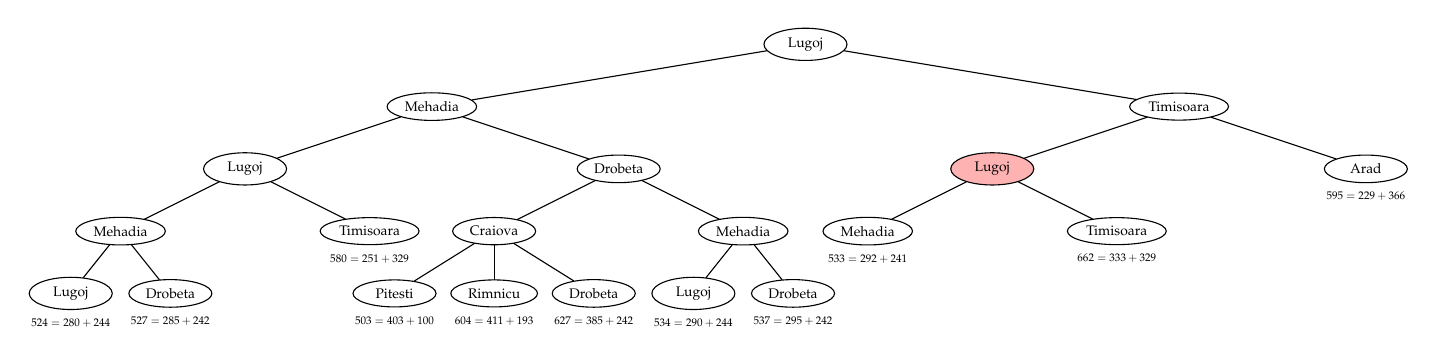
\begin{tikzpicture}[scale = 0.45]
            \node [normal] (L) {Lugoj}
                child {node [normal] (M) {Mehadia}
                    child {node [normal] (L2) {Lugoj}
                        child {node [normal] (M2) {Mehadia}
                            child {node [normal] (L4) {Lugoj}}
                            child {node [normal] (D3) {Drobeta}}
                        }
                        child {node [normal] (T2) {Timisoara}}
                    }
                    child {node [normal] (D) {Drobeta}
                        child {node [normal] (C) {Craiova}
                            child {node [normal] (P) {Pitesti}}
                            child {node [normal] (R) {Rimnicu}}
                            child {node [normal] (D2) {Drobeta}}
                        }
                        child {node [normal] (M3) {Mehadia}
                            child {node [normal] (L5) {Lugoj}}
                            child {node [normal] (D4) {Drobeta}}
                        }
                    }
                }
                child {node [normal] (T) {Timisoara}
                    child {node [expand] (L3) {Lugoj}
                        child {node [normal] (M4) {Mehadia}}
                        child {node [normal] (T3) {Timisoara}}
                    }
                    child {node [normal] (A) {Arad}}
                };

            \node [length, below = 0.2em of L4] (dL4) {$524 = 280 + 244$};
            \node [length, below = 0.2em of D3] (dD3) {$527 = 285 + 242$};
            \node [length, below = 0.2em of T2] (dT2) {$580 = 251 + 329$};
            \node [length, below = 0.2em of L5] (dL5) {$534 = 290 + 244$};
            \node [length, below = 0.2em of D4] (dD4) {$537 = 295 + 242$};
            \node [length, below = 0.2em of P] (dP) {$503 = 403 + 100$};
            \node [length, below = 0.2em of R] (dR) {$604 = 411 + 193$};
            \node [length, below = 0.2em of D2] (dD2) {$627 = 385 + 242$};
            \node [length, below = 0.2em of M4] (dM4) {$533 = 292 + 241$};
            \node [length, below = 0.2em of T3] (dT3) {$662 = 333 + 329$};
            \node [length, below = 0.2em of A] (dA) {$595 = 229 + 366$};
        \end{tikzpicture}
    }

    \subfigure
    {
        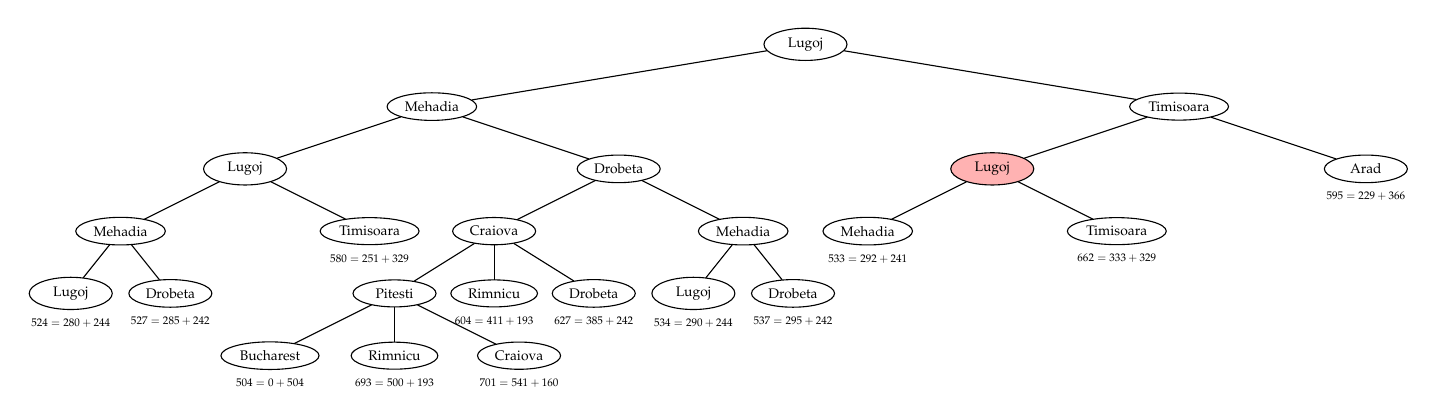
\begin{tikzpicture}[scale = 0.45]
            \node [normal] (L) {Lugoj}
                child {node [normal] (M) {Mehadia}
                    child {node [normal] (L2) {Lugoj}
                        child {node [normal] (M2) {Mehadia}
                            child {node [normal] (L4) {Lugoj}}
                            child {node [normal] (D3) {Drobeta}}
                        }
                        child {node [normal] (T2) {Timisoara}}
                    }
                    child {node [normal] (D) {Drobeta}
                        child {node [normal] (C) {Craiova}
                            child {node [normal] (P) {Pitesti}
                                child {node [normal] (B) {Bucharest}}
                                child {node [normal] (R2) {Rimnicu}}
                                child {node [normal] (C2) {Craiova}}
                            }
                            child {node [normal] (R) {Rimnicu}}
                            child {node [normal] (D2) {Drobeta}}
                        }
                        child {node [normal] (M3) {Mehadia}
                            child {node [normal] (L5) {Lugoj}}
                            child {node [normal] (D4) {Drobeta}}
                        }
                    }
                }
                child {node [normal] (T) {Timisoara}
                    child {node [expand] (L3) {Lugoj}
                        child {node [normal] (M4) {Mehadia}}
                        child {node [normal] (T3) {Timisoara}}
                    }
                    child {node [normal] (A) {Arad}}
                };

            \node [length, below = 0.2em of L4] (dL4) {$524 = 280 + 244$};
            \node [length, below = 0.2em of D3] (dD3) {$527 = 285 + 242$};
            \node [length, below = 0.2em of T2] (dT2) {$580 = 251 + 329$};
            \node [length, below = 0.2em of L5] (dL5) {$534 = 290 + 244$};
            \node [length, below = 0.2em of D4] (dD4) {$537 = 295 + 242$};
            \node [length, below = 0.2em of B] (dB) {$504 = 0 + 504$};
            \node [length, below = 0.2em of R2] (dR2) {$693 = 500 + 193$};
            \node [length, below = 0.2em of C2] (dC2) {$701 = 541 + 160$};
            \node [length, below = 0.2em of R] (dR) {$604 = 411 + 193$};
            \node [length, below = 0.2em of D2] (dD2) {$627 = 385 + 242$};
            \node [length, below = 0.2em of M4] (dM4) {$533 = 292 + 241$};
            \node [length, below = 0.2em of T3] (dT3) {$662 = 333 + 329$};
            \node [length, below = 0.2em of A] (dA) {$595 = 229 + 366$};
        \end{tikzpicture}
    }
    \caption{使用A$^*$搜索应用直线距离启发式求解从 Lugoj 到 Bucharest 问题(续)}
    \label{figure:2}
\end{figure}
\restoregeometry

\section{Exercise 3.25}
\textbf{启发式路径算法}(Pohl,1977)是一种最佳优先搜索,它的评估函数是$f(n) = (2 - w)g(n) + wh(n)$,假设 $h$ 是可采纳的。$w$取什么值能保证算法是最优的?当$w = 0,\ w = 1,\ w = 2$时,分别是什么搜索算法?

\paragraph{解}
由于 $h$ 是可采纳的,为了保证一致性,应有:
\begin{equation*}
    \left\{
        \begin{aligned}
            & 2 - w > 0 \\
            & w \geq 0
        \end{aligned}
    \right.
\end{equation*}
同时成立,即 $0 \leq w < 2$ 时算法是最优的。

当$w = 0$时,$f(n) = 2g(n)$,算法退化为(带有常系数的)一致代价搜索;当$w = 1$时,$f(n) = g(n) + h(n)$,算法即A$^*$搜索;当$w = 2$时,算法是(带有常系数的)贪婪最佳优先搜索。

\section{Exercise 3.28}
设计一个启发函数,它在八数码问题中有时会估计过高,并指出对某一特定问题它会求出次优解(可以用计算机编程找出)。证明:如果$h$被高估的部分不超过$c$,A$^*$算法返回的解代价比最优解代价多出的部分也不超过$c$。

\paragraph{解}
启发式函数为不在位的棋子数与所有棋子到其目标位置的曼哈顿距离和之和,即$h = h_1 + h_2$。对于如图\ref{figure:2}的状态
\begin{figure}[h]
    \centering
    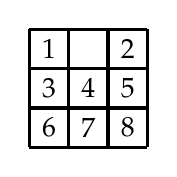
\begin{tikzpicture}[scale=.5]
        \begin{scope}
          \draw[very thick] (0, 0) grid (3, 3);
          \setcounter{row}{1}
          \setrow {1}{ }{2}
          \setrow {3}{4}{5}
          \setrow {6}{7}{8}
        \end{scope}
    \end{tikzpicture}
    \label{figure:2}
    \caption{一个在八数码问题中估计过高的实例}
\end{figure}
其启发式函数为$h = 1 + 1 = 2$,高于其实际的解代价1。
\begin{proof}
    设$h$被高估的部分不超过$c$,即$h(n) \leq h^*(n) + c$,则对于最优解路径上的任意结点$n$,有
    \begin{align*}
        f(n) = & g(n) + h(n) \\
        \leq & g(n) + h^*(n) + c \\
        \leq & C^* + c
    \end{align*}
    即A$^*$算法返回的解代价比最优解代价多出的部分也不超过$c$。
\end{proof}

\section{Exercise 3.29}
证明如果启发式是一致的,它一定是可采纳的。构造一个非一致的可采纳启发式。

\paragraph{解}
设启发式$h(n)$是一致的,即对于每个结点$n$和通过任一行动$a$生成的$n$的每个后继结点$n'$,从结点$n$到达目标的估计代价不大于从$n$到$n'$的单步代价与从$n'$到达目标的估计代价之和:$$h(n) \leq c(n,\, a,\, n') + h(n')$$
\begin{proof}
    对从$n$到任何目标的最短路径上的结点数$k$进行归纳:

    当$k = 1$时,取目标结点即$n'$,则$h(n) \leq c(n,\, a,\, n') + h(n')$成立。

    当$k \leq 1$时,假设$h(n')$是可采纳的,则有
    \begin{equation*}
        h(n) \leq c(n,\, a,\, n') + h(n') \leq c(n,\, a,\, n') + h^*(n') = h^*(n)
    \end{equation*}
    即$h(n)$对$k + 1$仍是可采纳的。

    综上,$h(n)$是可采纳的。
\end{proof}
在 Romania 问题中,如果使用到达 Bucharest 的最少经过一个中间结点的路径距离减去到达后继结点的最大直线距离作为启发式,这个启发式是非一致的,它并不满足三角不等式,但它仍不会给出过高的估计,因此是可采纳的。

\section{Exercise 6.5}
使用带前向检验、MRV和最少约束值启发式的回溯算法手动求解图中的密码算术问题
\begin{figure}[h]
    {
        \centering
        \subfigure[]{
            \includegraphics[]{Figure6-2(a).png}
        }
        \subfigure[]{
            \includegraphics[]{Figure6-2(b).png}
        }
        \caption{}
    }
    (a) 密码算术问题。不同字母表示不同的数字;目标是找到能够使加法算式成立的代替字母的数字,附加约束是最前面的数字不能是0。 (b) 密码算术的约束超图,给出的是 \textit{Alldiff} 约束(最上方的方框)和每列的相加约束(中间的四个方框)。变量$C_1$、$C_2$、$C_3$表示每列进位
\end{figure}

\paragraph{解}
手动求解过程如下:
\begin{enumerate}[i]
    \item 选择变量$C_3$,其表示进位,因此有$C_3 \in \{0,\, 1\}$
    \item 取$C_3 = 1$,由前向检验限制,附加约束是最前面的数字不能是0,因此$F$不能取0,故$C_3$不能取0
    \item 选择变量$F$,其只有一个可能的值
    \item 取$F = 1$
    \item 选择变量$C_2$,其有两个可能的值
    \item 取$C_2 = 0$
    \item 选择变量$X_1$,其现在只有一个可能的值
    \item 取$C_1 = 0$
    \item 选择变量$O$,由于$O + O = R + 10 \times C_1 = R \leq 9$,且$T + T = O + 10 \times F = O + 10$,因此$O$是小于5的偶数,这是最严格的约束
    \item 取$O = 4$
    \item 选择变量$R$,其现在只有一个可能的值
    \item 取$R = 8$
    \item 选择变量$T$,其现在只有一个可能的值
    \item 取$T = 7$
    \item 选择变量$U$,由于$W + W = U + 10 \times C_2 = U \leq 9$,因此$U$是小于9的偶数
    \item 取$U = 6$,由前向检验限制,不同的字母表示不同的数字,因此$U$不能取$4$或$8$
    \item 选择变量$W$,其现在只有一个可能的值
    \item 取$W = 3$
    \item 得到一个解:$F = 1,\ T = 7,\ U = 6,\ W = 3,\ R = 8,\ O = 4$
\end{enumerate}

\section{Exercise 6.11}
用 AC-3 算法说明弧相容对图中问题能够检测出部分赋值$\{WA = red,\ V = blue\}$的不相容
\begin{figure}[h]
    {
        \centering
        \subfigure[]{
            \includegraphics[scale = 0.6]{Figure6-1(a).png}
        }
        \subfigure[]{
            \includegraphics[scale = 0.6]{Figure6-1(b).png}
        }
        \caption{着色问题}
    }
    (a) 澳大利亚的洲和行政区。视此地图着色问题为约束满足问题(CSP)。目标是对每个区域分配颜色,使得相邻的区域不同色。 (b) 将地图着色问题表示成约束图
\end{figure}

\paragraph{解}
以下列出了 AC-3 算法的执行过程:
\begin{enumerate}[i]
    \item 删除边\textit{SA}-\textit{WA},从\textit{SA}的值域中删除\textit{green},剩余\{\textit{red}, \textit{blue}\}
    \item 删除边\textit{SA}-\textit{V},从\textit{SA}的值域中删除\textit{red},剩余\{\textit{blue}\}
    \item 删除边\textit{NT}-\textit{WA},从\textit{NT}的值域中删除\textit{green},剩余\{\textit{red}, \textit{blue}\}
    \item 删除边\textit{NT}-\textit{SA},从\textit{NT}的值域中删除\textit{blue},剩余\{\textit{red}\}
    \item 删除边\textit{NSW}-\textit{SA},从\textit{NSW}的值域中删除\textit{blue},剩余\{\textit{red}, \textit{green}\}
    \item 删除边\textit{NSW}-\textit{V},从\textit{NSW}的值域中删除\textit{green},剩余\{\textit{green}\}
    \item 删除边\textit{Q}-\textit{NT},从\textit{Q}的值域中删除\textit{red},剩余\{\textit{blue}, \textit{green}\}
    \item 删除边\textit{Q}-\textit{SA},从\textit{Q}的值域中删除\textit{blue},剩余\{\textit{green}\}
    \item 删除边\textit{Q}-\textit{NSW},从\textit{Q}的值域中删除\textit{green},剩余$\varnothing$,返回\texttt{false}
\end{enumerate}
因此部分赋值$\{WA = red,\ V = blue\}$不相容。

\section{Exercise 6.12}
用 AC-3 算法求解树结构 CSP 在最坏情况下的复杂度是多少?

\paragraph{解}
在树结构 CSP 中,最坏情况下,考虑每一条弧各一次,因此算法的复杂度是$O(ED)$,其中$E$是树结构中边的数量,$D$是最大的域的大小
\end{document}